% !TEX root = ../../main.tex
\section{Data Gathering}\label{sec:data_gathering}

\TODO{These plots should be in }

%---- Run 1: walk-run-roemer
\begin{figure}
\centering
  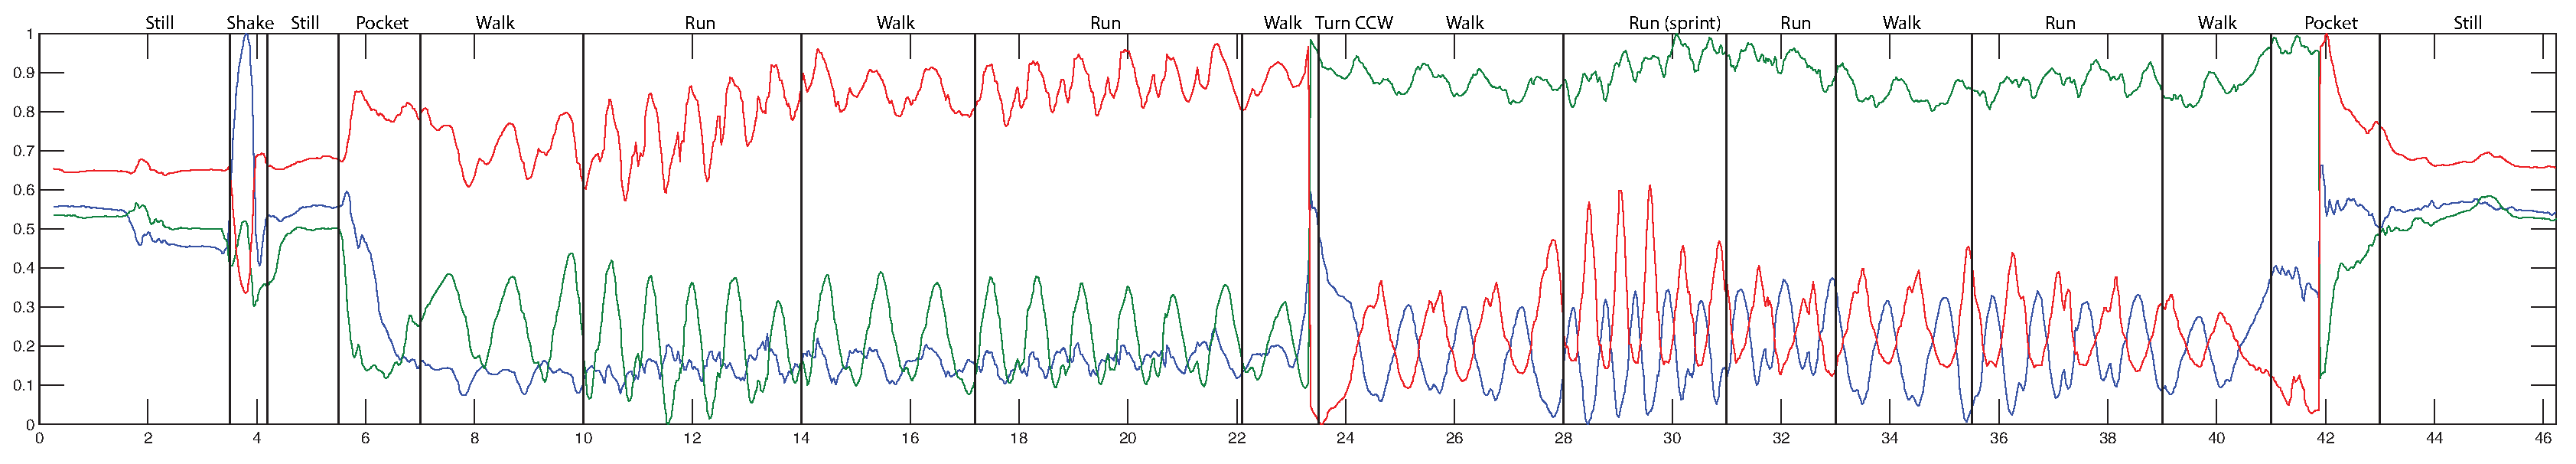
\includegraphics[width=1\textwidth]{./Figures/chapter6/data_collection/run-1-walk-run-roemer/data_plot_rot_annotated.eps}
  \caption[R1: rotation]{Run 1: Walk-run-roemer, rotation}
\end{figure}

\begin{figure}
\centering
  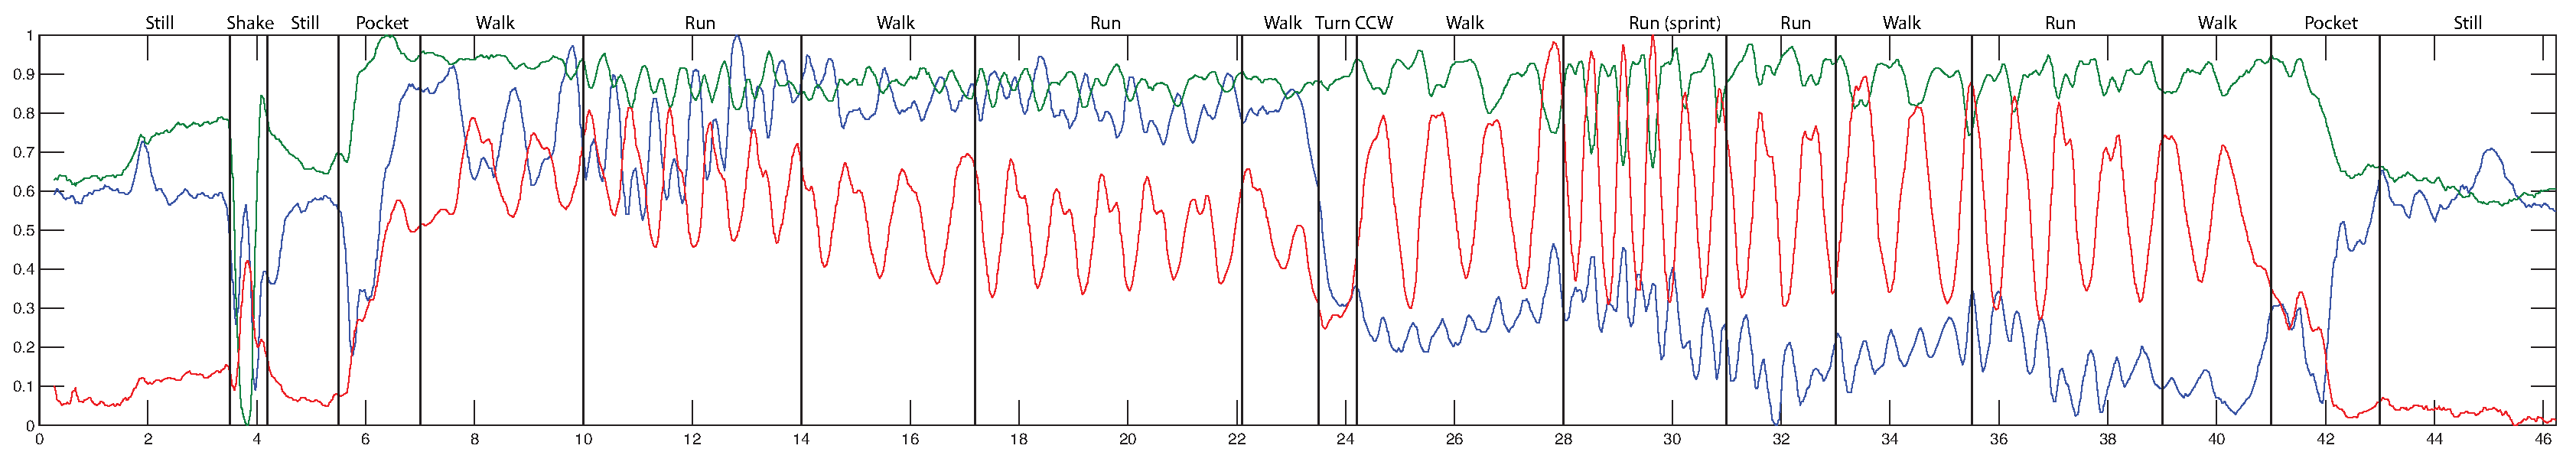
\includegraphics[width=1\textwidth]{./Figures/chapter6/data_collection/run-1-walk-run-roemer/data_plot_mag_annotated.eps}
  \caption[R1: mag]{Run 1: Walk-run-roemer, Mag}
\end{figure}

\begin{figure}
\centering
  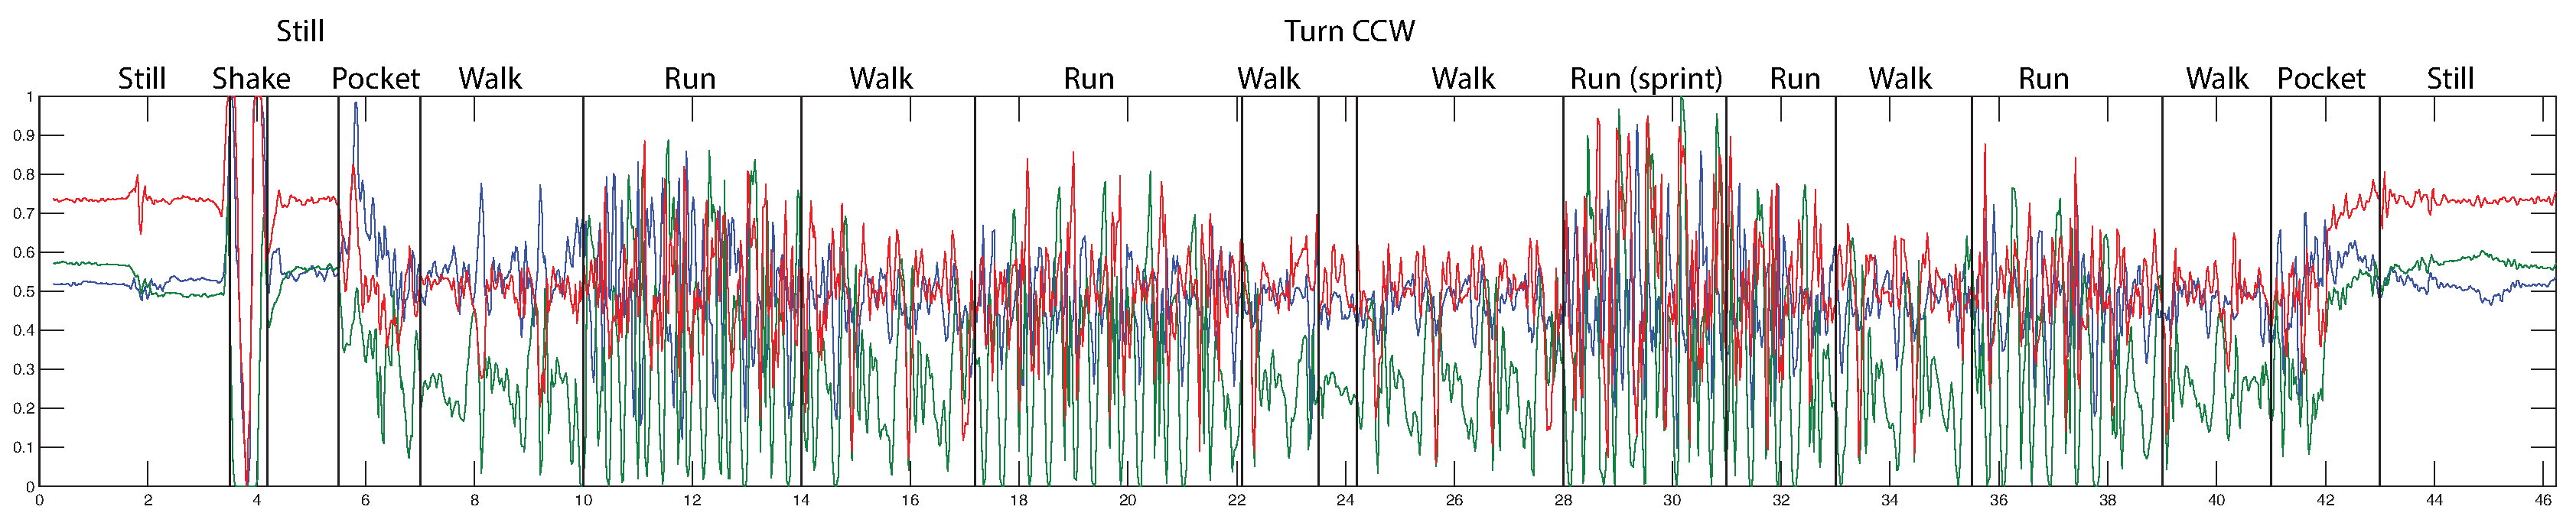
\includegraphics[width=1\textwidth]{./Figures/chapter6/data_collection/run-1-walk-run-roemer/data_plot_acc_annotated.eps}
  \caption[R1: accelerometer]{Run 1: Walk-run-roemer, accelerometer}
\end{figure}

%---- Run 2: walk-run-jos
\begin{figure}
\centering
  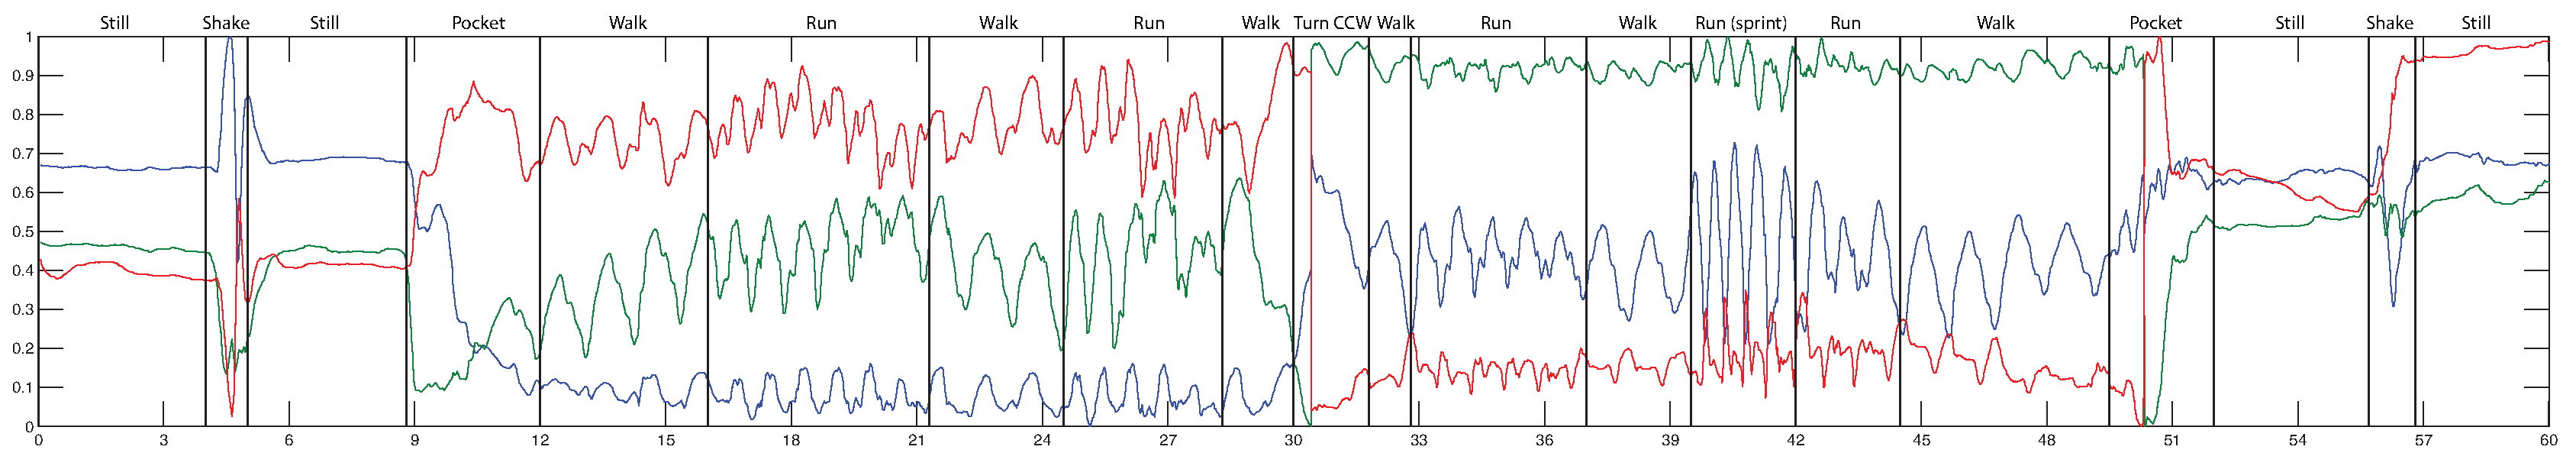
\includegraphics[width=1\textwidth]{./Figures/chapter6/data_collection/run-2-walk-run-jos/data_plot_rot_annotated.eps}
  \caption[R2: rotation]{Run 2: Walk-run-jos, rotation}
\end{figure}

\begin{figure}
\centering
  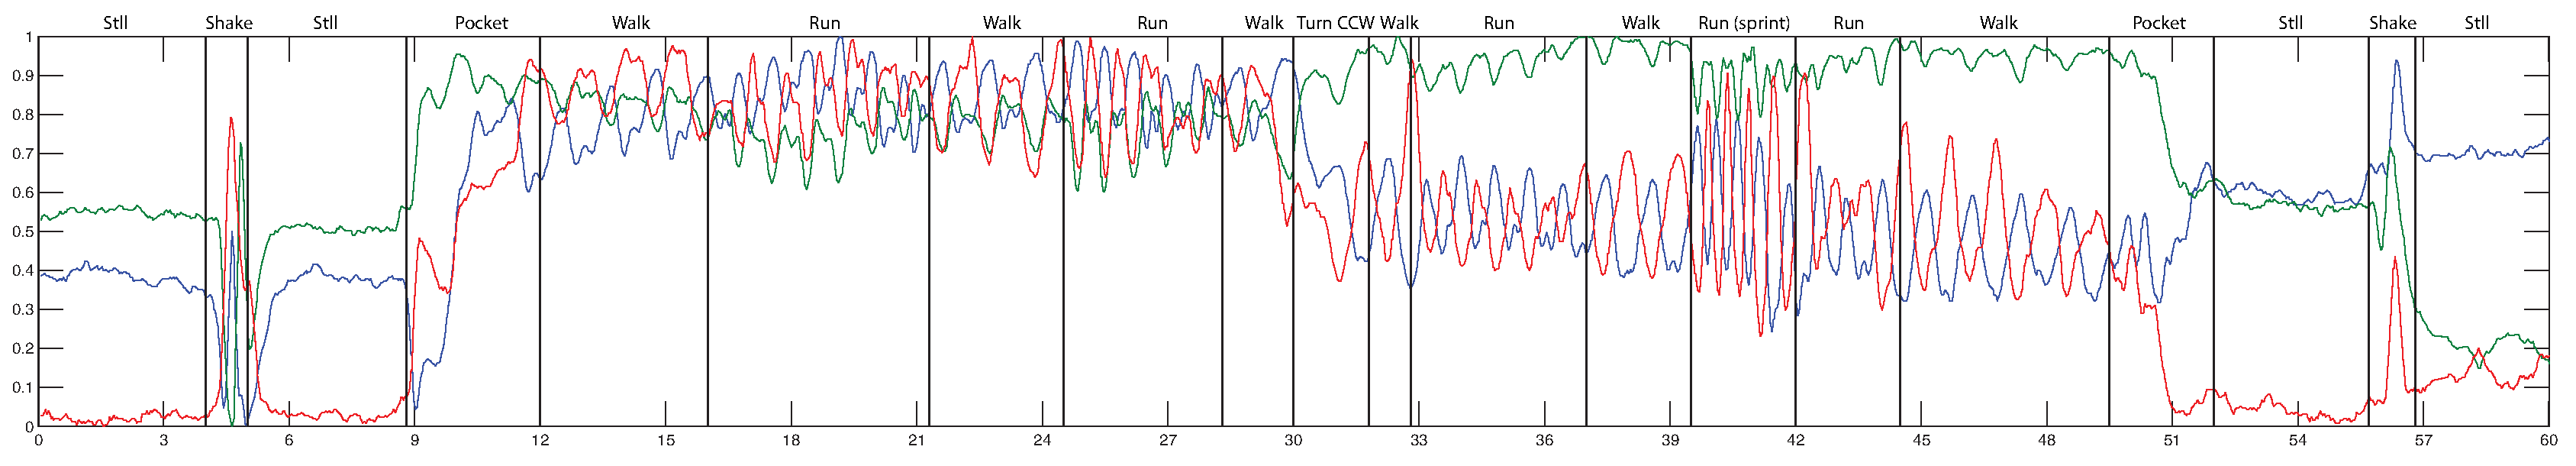
\includegraphics[width=1\textwidth]{./Figures/chapter6/data_collection/run-2-walk-run-jos/data_plot_mag_annotated.eps}
  \caption[R2: mag]{Run 2: Walk-run-jos, Mag}
\end{figure}

\begin{figure}
\centering
  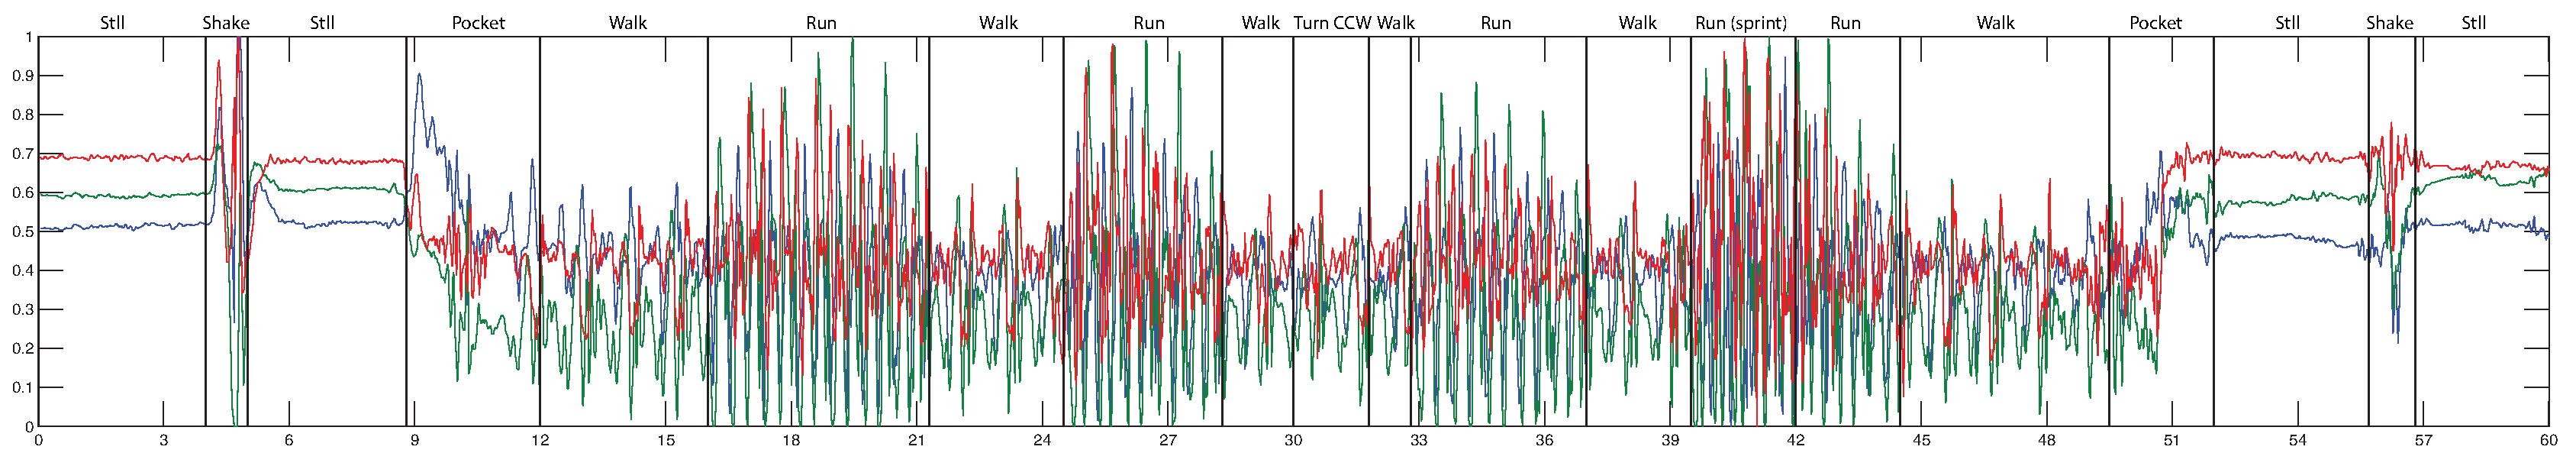
\includegraphics[width=1\textwidth]{./Figures/chapter6/data_collection/run-2-walk-run-jos/data_plot_acc_annotated.eps}
  \caption[R2: accelerometer]{Run 2: Walk-run-jos, accelerometer}
\end{figure}